% MA211 - Lecture 15
\documentclass[pdftex, xcolor=pdftex, dvipsnames,handout]{beamer}

\usetheme{MA211}
\usepackage{thumbpdf}
\usepackage{wasysym}
%\usepackage{ucs}
\usepackage[utf8]{inputenc}
\usepackage{pgf,pgfarrows,pgfnodes,pgfautomata,pgfheaps,pgfshade}
\usepackage{verbatim}

\usepackage{eurosym}
\usepackage{euler}

\usepackage{calc}               % Simple computations with LaTeX variables
%\usepackage[hang]{caption2}     % Improved captions

\usepackage{graphicx}           % Standard graphics package

\usepackage{amsmath, amsthm, amssymb}


\newcommand{\fquad}{\mbox{\qquad}}
\newcommand{\bull}{$\bullet$ }

\newcommand {\I} {\mathcal I}
\newcommand {\calI} {\mathcal I}
\def\disint{\displaystyle\int}

\DeclareMathOperator{\D}{d}
\newcommand{\dydx}{\frac{\D y}{\D x}}

%\definecolor{gray}{rgb}{0.69, 0.69, 0.69} \newcommand{\gray}[1]{\textcolor{gray}{#1}}
\definecolor{dogreen}{rgb}{0.33, 0.42, 0.18} \newcommand{\dogreen}[1]{\textcolor{dogreen}{#1}}
\definecolor{maroon}{rgb}{.5,0.2,0.2}\newcommand{\maroon}[1]{\textcolor{maroon}{#1}}
\definecolor{greena}{rgb}{.1,0.581,0.1}\newcommand{\greena}[1]{\textcolor{greena}{#1}}

\definecolor{blue4}{rgb}{0,0,.545}
\newcommand{\Blue}[1]{\textcolor{blue}{#1}}
\newcommand{\Red}[1]{\textcolor{red}{#1}}
\definecolor{pink}{rgb}{1.,0.75,0.8}
\definecolor{darkred}{rgb}{0.5,0.0,0.0}
\definecolor{darkgreen}{rgb}{0,0.3,0.3}
\definecolor{purple}{rgb}{0,0.3,0.3}
\definecolor{darkblue}{rgb}{0.0, 0.0, .5}
\definecolor{dpurple}{rgb}{.3,.0,.3}
\newcommand{\Green}[1]{\textcolor{darkgreen}{#1}}
\newcommand{\DRed}[1]{\textcolor{darkred}{#1}}
\newcommand{\DBlue}[1]{\textcolor{darkblue}{#1}}
\newcommand{\Purple}[1]{\textcolor{dpurple}{#1}}
\newcommand{\Emph}[1]{\textcolor{darkred}{\textbf{\it #1}}}
\newcommand{\remph}[1]{\textcolor{darkred}{\textbf{\emph{#1}}}}
\newcommand{\bemph}[1]{\textcolor{darkblue}{\textbf{\emph{#1}}}}
\newcommand{\gemph}[1]{\textcolor{darkgreen}{\textbf{\emph{#1}}}}
\newcommand{\Bf}[1]{\textcolor{darkblue}{\textbf{#1}}}
\newcommand{\Gf}[1]{\textcolor{darkgreen}{\textbf{#1}}}
\newcommand{\Rf}[1]{\textcolor{red}{\textbf{#1}}}
\newcommand{\Rmf}[1]{\textcolor{red}{\mathbf{#1}}}

\newcommand{\Conj}[1]{\overline{#1}}

\newcommand{\code}[1]{\textcolor{darkblue}{\texttt{\textbf{#1}}}}
\newcommand{\icode}[1]{{\blue\texttt{\textbf{\emph{#1}}}}}
\newcommand{\gcode}[1]{{\Green{\texttt{\textbf{\emph{#1}}}}}}
\newcommand{\out}[1]{\texttt{\emph{\textbf{\Green{#1}}}}}





\newenvironment{vminipage}%
{\begin{Sbox}\begin{minipage}\begin{small}\begin{verbatim}}%
{\end{verbatim}\end{small}\end{minipage}\end{Sbox}\fbox{\TheSbox}}

\newenvironment{nminipage}%
{\begin{Sbox}\begin{minipage}}%
{\end{minipage}\end{Sbox}\fbox{\TheSbox}}


\let\Arg\relax\DeclareMathOperator{\Arg}{\mathtt{Arg}}
\let\Arg\relax\DeclareMathOperator{\e}{\mathtt{e}}

\newcommand {\AND} {\wedge}
\newcommand {\OR} {\vee}
\newcommand {\NOT} {\neg}
\newcommand {\IMPLIES} {\rightarrow}
%\newcommand {\IFF} {\leftrightarrow}
\renewcommand {\iff} {\Leftrightarrow}
\newcommand {\NAND} {\uparrow}
\newcommand {\NOR} {\downarrow}
\newcommand {\XOR} {\otimes}

\newenvironment{citemize}% Colour items
{\begin{description}}%
{\end{description}}

\newcommand {\maroonitem}{\item[\maroon{$\bullet$}]}

\newcommand {\gitem} {\item {\includegraphics[width=.4cm,angle=-10]{img/green-bullet-on-white.ps}}}
\newcommand {\ritem} {\item {\includegraphics[width=.4cm,angle=-10]{img/red-bullet-on-white.ps}}}
\newcommand {\yitem} {\item {\includegraphics[width=.4cm,angle=-10]{img/yellow-bullet-on-white.ps}}}
\newcommand {\bitem} {\item {\includegraphics[width=.4cm,angle=-10]{img/blue-bullet-on-white.ps}}}

\newcommand {\greenitem} {\item {\includegraphics[width=.4cm,angle=-10]{img/green-bullet-on-white.ps}}}
\newcommand {\reditem} {\item {\includegraphics[width=.4cm,angle=-10]{img/red-bullet-on-white.ps}}}
\newcommand {\yellowitem} {\item {\includegraphics[width=.4cm,angle=-10]{img/yellow-bullet-on-white.ps}}}
\newcommand {\blueitem} {\item {\includegraphics[width=.4cm,angle=-10]{img/blue-bullet-on-white.ps}}}

\newcommand {\eq}[1]%
  {$\DBlue{#1}$}
\newcommand {\eqd}[1]%
  {$\displaystyle\DBlue{#1}$}
%\newcommand{\eq}[1]{\boldmath \DBlue{$#1$}}


\newcommand {\csf}{\centerslidesfalse}
\newcommand {\cst}{\centerslidestrue}

\newcommand {\vecii}[2] {   \big(\begin{smallmatrix} #1 \\ #2 \end{smallmatrix}\big)}
\newcommand{\atwo}[2]{\left(\!\!\begin{array}{c} #1 \\ #2 \end{array}\!\!\right)}


\newcommand{\C}{\mathbb{C}}
\newcommand{\Q}{\mathbb{Q}}
\newcommand{\R}{\mathbb{R}}
\newcommand{\N}{\mathbb{N}}
\newcommand{\Z}{\protect\mathbb{Z}}  % protect for index.
\newcommand {\Rs}{ \mathbb{R}}
\newcommand {\Cs}{ \mathbb{C}}
\newcommand {\Rnn}{ \mathbb{R}^{n \times n}}
\newcommand {\Rn}{ \mathbb{R}^{n}}


\newcommand{\mblock}{%
\setbeamercolor*{block title}{bg=maroon,fg=white}
\setbeamercolor*{block body}{bg=white,fg=maroon}
}%

\newcommand{\bblock}{%
\setbeamercolor*{block title}{bg=Steel,fg=white}
\setbeamercolor*{block body}{bg=Mylightgray,fg=Steel}
}%

\newcommand{\gblock}{%
\setbeamercolor*{block title}{bg=Green,fg=white}
\setbeamercolor*{block body}{bg=Mylightgray,fg=darkgreen}
}%


\newcommand{\rblock}{%
\setbeamercolor*{block title}{bg=Red,fg=white}
\setbeamercolor*{block body}{bg=white,fg=Black}
}%


\newcommand{\TakeNotes}{
\includegraphics[width=2cm]{TakeNote}}

\def\eps{\varepsilon}
\newcommand {\del}[2]{ {\frac{\partial #1}{\partial #2}}}
\newcommand {\x}[1]{x^{[#1]}}
\newcommand {\delx}{ {\frac{\partial}{\partial x}}}
\newcommand {\delt}{ {\frac{\partial}{\partial t}}}
\newcommand {\dely}{ {\frac{\partial}{\partial y}}}
\newcommand {\ith}{{(i)}}
\renewcommand {\vec}[1]{ {\boldsymbol{#1}}}
\newcommand {\Oh} {\mathcal O}
\newcommand {\Err} {\mathcal E}
%\newcommand {\th} {\mathrm{th}}
\DeclareMathOperator{\fl}{fl}
\DeclareMathOperator{\sign}{sign}
\DeclareMathOperator{\Cond}{Cond} 
\DeclareMathOperator{\cond}{cond}
\DeclareMathOperator{\diag}{diag} 
\DeclareMathOperator{\sym}{sym} 
\DeclareMathOperator{\Trace}{Trace}
%\DeclareMathOperator{\D}{d}
\DeclareMathOperator{\E}{e}

\newcommand {\Rsym}{{ \mathbb{R}^{n \times n}_\mathrm{sym}}}

\newcommand {\st} {\mathrm{st}}
\newcommand {\nd} {\mathrm{nd}}


\parskip .25cm


\theoremstyle{definition}
\newtheorem{exercise}{Exercise}[section]
\newtheorem{method}{Method}[section]

\newcommand{\Header}[1]{\begin{center}{\Large \Bf{#1}}\end{center}}

\subtitle{MA211}
\title{Lecture 15: Nonhomogeneous $2^\mathrm{nd}$-order DEs (final part). Series Solutions}

\author{Dr Niall Madden}

\date{\Large Wed $29^\mathrm{th}$ October  2008}


\begin{document}

\setcounter{framenumber}{-1}
\frame{

\begin{block}{}
\begin{center}
{\large \insertsubtitle}

\vspace{.1cm}

\begin{large}
\textbf{\inserttitle}
\end{large}

\vspace{.15cm}

% {\footnotesize \insertauthor}

\vspace{.3cm}

{ {\insertdate}}
\end{center}
\end{block}


\vspace{-0.25cm}
\begin{center}
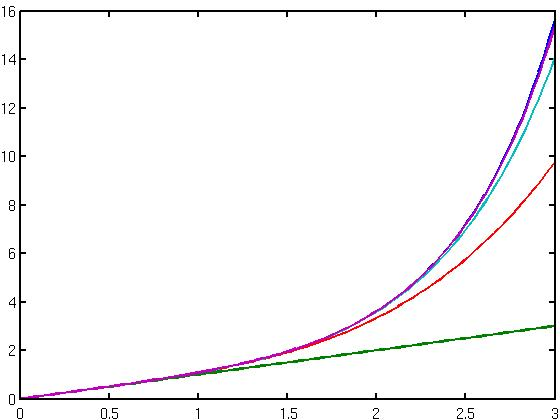
\includegraphics[height=4cm]{images/Series4}
\end{center}
}




\frame{
  \frametitle{Today...}

 \tableofcontents


For further details and examples, look at the section on
\Emph{Nonhomogeneous Linear Equations}, Section 17.2 of Stewart
\Emph{Calculus: early transcendentals}.

}



\frame{
So far we have studied how to find general solutions to the following
types of problems:
\begin{block}{}
\hspace{2cm} \eq{  ay'' + by' + cy = \alert{1 +2x^2 + 3x^4}}.\\ 
\hspace{2cm} \eqd{ ay'' + by' + cy =  \alert{e^{-x/2}}}.\\ 
\hspace{2cm} \eq{  ay'' + by' + cy = \alert{\sin(3 x)}}.
\end{block}


Then we moved onto ones of the form:
\begin{block}{}
\hspace{2cm} \eq{  ay'' + by' + cy = \alert{P(x) + e^{Tx} +
    \cos(\omega x)}},\\
proceeding by solving each of \\
\hspace{2cm} \eq{  ah'' + bh' + ch = \alert{0}};\\
\hspace{2cm} \eq{  au'' + bu' + cu = \alert{P(x)}};\\
\hspace{2cm} \eq{  av'' + bv' + cv = \alert{e^{Tx}}}.\\
\hspace{2cm} \eq{  aw'' + bw' + cw = \alert{\cos(\omega x)}}.\\
Then the general solution will be\\
\hspace{2cm} \eqd{y(x) = h(x) + u(x) + v(x) + w(x).}
\end{block}
}


\section{$f$ is the product of two functions}
\frame{
Finally we will consider how to solve problems with the form:
\begin{block}{}
\hspace{2cm} \eq{  ay'' + by' + cy = \alert{P(x)e^{Tx}}},\\
\hspace{2cm} \eq{  av'' + bv' + cv = \alert{P(x)\sin(Tx)}}.\\
where \eq{T} is some real number and \eq{P(x)} is a polynomial of
degree \eq{x}.
\end{block}

}

\subsection{$f(x) = P(x)e^{Tx}$}
\frame{
To find the solution to 
\begin{block}{}
\[   ay'' + by' + cy = \alert{P(x)e^{Tx}} \]
where \eq{P} is a polynomial of degree \eq{n}.
\end{block}
\begin{itemize}
\item Let \eq{h} be the general solution to 
\eqd{ ah'' + bh' + ch =0.}
\item Let \eq{u} be one of 
\begin{itemize}
\item  \eq{(q_0 + q_1x + \cdots + q_nx^n)e^{Tx}}, if $T$ is not a
  solution to the auxiliary equation.

\item  \eqd{(q_0 + q_1x + \cdots + q_nx^n)\alert{x}e^{Tx}}, if the auxiliary
  equation has two solutions, one of which is $T$.

\item  \eqd{(q_0 + q_1x + \cdots + q_nx^n)\alert{x^2}e^{Tx}}, if $T$ is the
  only solution to the auxiliary equation.
\end{itemize}
\item Substitute \eq{u} into
\[   au'' + bu' + cu' = \alert{P(x)e^{Tx}},\]
  divide by \eq{e^{Tx}} and solve for \eq{q_n}, \eq{q_{n-1}},
  \eq{\dots}, \eq{q_0}. 


\end{itemize}
}

\frame{

\begin{example}
Find the general solution to the non-homogeneous problem:
\[ y'' - 4y' + 4y = x^2e^x.\]
\end{example}
\vspace{4cm}
}

\section{$f(x) = P(x)\sin(x)$ or  $ P(x)\cos(x)$ }
\frame{
To find the solution to 
\begin{block}{}
\[   ay'' + by' + cy = \alert{P(x)\cos(Tx)} \]
where \eq{P} is a polynomial of degree \eq{n}.
\end{block}
\begin{itemize}
\item Let \eq{h} be the general solution to 
\[ ah'' + bh' + ch =0.\]
\item Let \eq{u = (A_0 +  A_1 x \cdots + A_nx^n)\cos(Tx)}\\
\hspace{3cm} \eq{+ (B_0 +  B_1 x \cdots + B_nx^n)\sin(Tx) }.
\item Substitute \eq{u} into the DE. Extract the equations for
  $\cos(Tx)$ and $\sin(Tx)$ .
\item Solve for \eq{A_n}, \eq{A_{n-1}},  \eq{\dots}, \eq{A_0}; 
\eq{B_n}, \eq{B_{n-1}},  \eq{\dots}, \eq{B_0}; 


\end{itemize}
}

\frame{

\begin{example}[Q4, Autumn, 06/07]
Find the general solution to the non-homogeneous problem:
\[ y'' + 2y = x \cos(x).\]
\end{example}
\vspace{4cm}
}

\frame{

\begin{exercise}[Q15.1]
Find general solutions to the following differential equations:
\begin{enumerate}
\item $y'' - 2y' + y = x + 1 + \sin(x)$
\item $y'' - 4y = x\sin(2x)$.
\item $y''  + 4y = 5 xe^{-x}$.
\end{enumerate}
\end{exercise}
}


\section{Power Series}

\frame{
We conclude this section with a note about \Bf{Power Series}.

We have a way of solving explicitly for problems with \Emph{constant
  coefficients}:
\[ a y'' + by' + cy = 0.\]

But for more general problems, such as,
\[
y'' + 2\alert{x}y'  + y=0,
\]
we have no such method.

However, we can find a very good \Emph{approximation} by using a
\Bf{Power Series}.

}


\frame{

\begin{alertblock}{Power Series}
The key idea is that we suppose that we can write \eq{y} as 
\[
y = c_0 + c_1 x + c_2x^2 + c_3x^3 + \cdots = \sum_{n=0}^\infty c_n
x^n.\]
\end{alertblock}

The general solution will always have arbitrary constants, so we let
these be \eq{c_0} and \eq{c_1}. 

Then we substitute the power series is into the differential equation, and get
equations for \eq{c_2}, \eq{c_3}, \eq{c_4}, ...

The more terms we take, the more accurate the solution is.
 

}

\frame{
\begin{example}
Find a Series Solution to 
\[y'' + y = 0,\]
where \eq{y=c_0 + c_1x + c_2x^2 + c_3 x^3 + c_4x^4 + c_5x^5}.
\end{example}


\vspace{4cm}

}

\frame{
This last example is not very typical. Usually we want a formula for
\Emph{all} of the coefficients \eq{c_2}, \eq{c_3}, \eq{c_4}, \dots.

Typically, for a second order problem, we get a formula for \eq{c_k}
in terms of \eq{c_k-2} that is called \Emph{recurrence relation}.

}



\frame{
\begin{example}
Find a recurrence relation for the coefficients of $c_0, c_1, c_2, \dots$,
of the series solution  \eqd{y= \sum_{n=0}^{\infty} c_n x^n} to
\[y'' + y = 0.\]

\end{example}


\vspace{4cm}

}

\end{document}
\frame{
\begin{example}
Use a power series to solve the DE
\[y'' - x y = 0.\]
\end{example}


\vspace{4cm}

}


\subsection{Initial Value problems}
\frame{
Power series methods are particularly useful for getting solutions to
\emph{initial value problems} where we are given, not only the
differential equation, but also the value of \eq{y} and \eq{y'} at
some initial point.

These allow us to solve for \eq{c_0} and \eq{c_1}.


}

\frame{
\begin{example}
Use a power series to solve the initial value problem
\[y'' - x y = 0, \qquad y(0)=0, y'(0)=1.\]
\end{example}


\vspace{4cm}

}

\frame{

\begin{center}
\only<5>{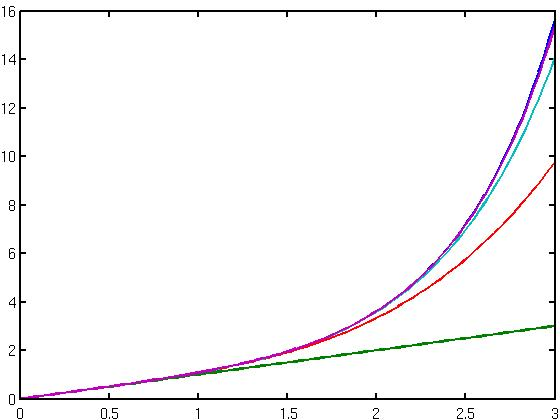
\includegraphics[height=7cm]{images/Series4}}
\only<1>{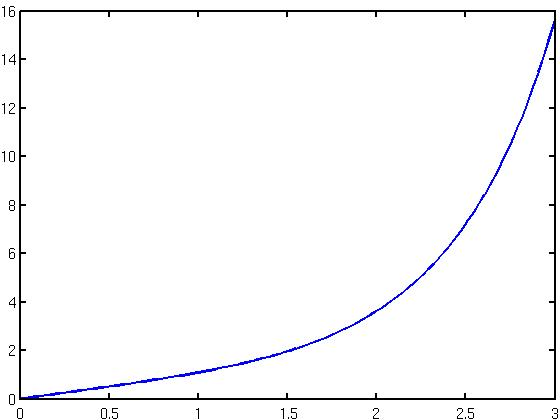
\includegraphics[height=7cm]{images/Series0}}
\only<2>{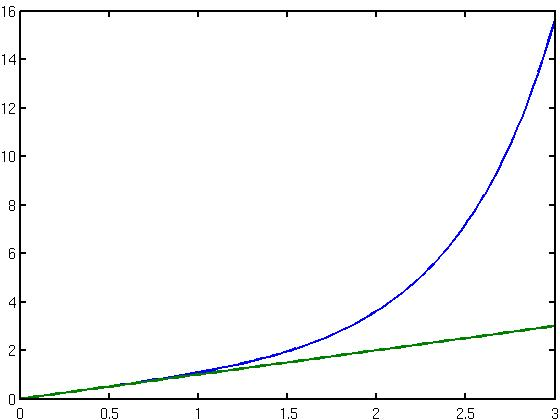
\includegraphics[height=7cm]{images/Series1}}
\only<3>{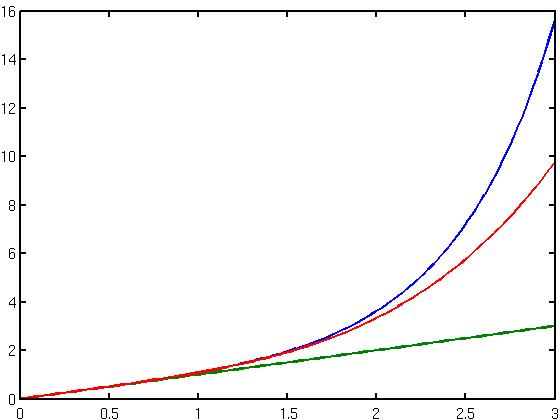
\includegraphics[height=7cm]{images/Series2}}
\only<4>{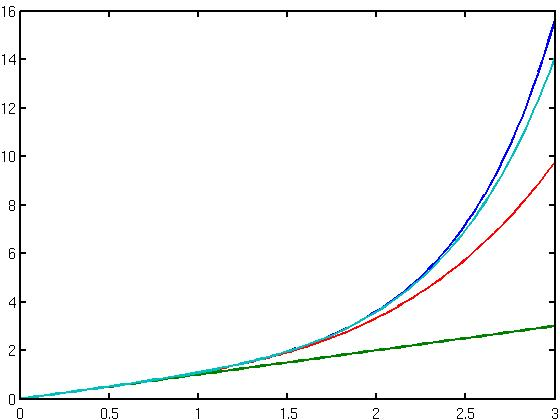
\includegraphics[height=7cm]{images/Series3}}
\end{center}

}
\frame{

\begin{exercise}[Q15.2]

For each of the following differential equations, find a recurrence
relation for the coefficients of  the power   series solution, and 
write out the solution up to the \eq{x^5} term.

\begin{enumerate}
\item $y'' + xy =0.$
\item $y'' + x^2 y =0.$

\item $y'' - 2xy' + y=0.$

\item $y'' - 2xy' + y=0, \quad y(0)=1, y'(0)=-1$

\item $y'' - xy' =0, \qquad y(0)=0, y'(0)=2$
\end{enumerate}



\end{exercise}
}



\end{document}

